% RESULTADOS-------------------------------------------------------------------

\chapter{Análise e Discussão dos Resultados}
\label{chap:resultados}

Este capítulo discute os resultados obtidos nos experimentos de detecção de cópias de vídeos através da aplicação das assinaturas digitais revisadas neste trabalho sobre os conjuntos de parametrização e teste detalhados na Seção~\ref{sec:met-Experimentos}.

Conforme detalhado na seção anterior, para a determinação do limiar de classificação de cada assinatura, são realizadas simulações de classificação utilizando um intervalo de limiares. Os casos de parametrização de cada assinatura são dividos em 5 subconjuntos e ao final, é utilizada a média dos limiares resultantes da simulação com cada subconjunto como limiar para a assinatura. Na Figura~\ref{fig:exemplo-simulacao}, foram plotados os valores de precisão, revocação e \textit{fmeasure} para cada assinatura ao longo das simulações com diferentes limiares. O ponto vermelho de cada sub-gráfico ilustra como é feita a escolha de um limiar para cada assinatura.

\begin{figure}[h]
	\centering
	\caption{Exemplo de simulação de classificação para um tipo de assinatura. O eixo X é composto dos limiares testados para a assinatura. O ponto vermelho indica o valor máximo de \textit{fmeasure}, ponto em que o limiar apresenta o melhor resultado.}
	\label{fig:exemplo-simulacao}
	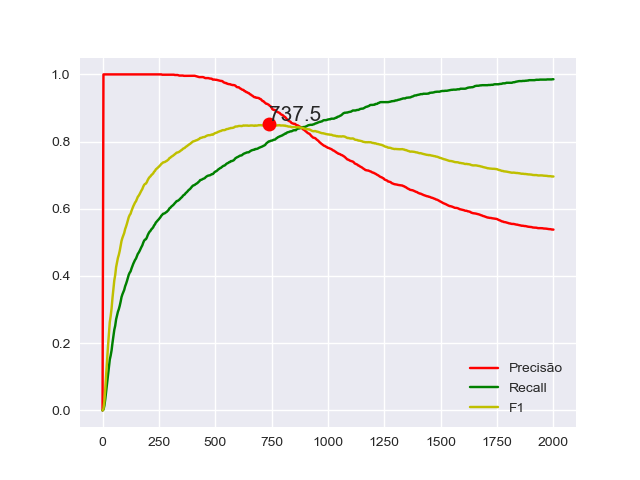
\includegraphics[width=\textwidth]{dados/figuras/experimentos/limiar_Medida_Ordinal_0.png}
    \fonte{Autoria própria.}
\end{figure}

Os subconjuntos de parametrização foram nomeados de T.1 a T.5 e o melhor limiar resultante da simulação com cada subconjunto está disposto na Tabela~\ref{tab:limiares}, além do limiar final de cada algoritmo.

\begin{table}[h]
	\caption{Limiares obtidos nas simulações com cada subconjunto de parametrização.}
	\label{tab:limiares}
	\begin{tabular}{|l|r|r|r|r|r|r|}
		\hline
		\textbf{Assinatura} & \textbf{T.1} & \textbf{T.2} & \textbf{T.3} & \textbf{T.4} & \textbf{T.5} & \textbf{Limiar Final}\\ \hline
		Gradiente & 761.52 & 637.27 & 681.36 & 705.41 & 629.25 & 682.96\\ \hline
		FrameDiff & 6.63 & 6.48 & 6.33 & 6.78 & 6.93 & 6.63\\ \hline
		Medida Ordinal & 657.31 & 729.45 & 661.32 & 725.45 & 749.49 & 704.60\\ \hline
		Wavelets & 597.19 & 593.18 & 625.25 & 601.20 & 625.25 & 608.41\\ \hline
		RBP & 5501.00 & 6793.58 & 6553.10 & 6147.29 & 4569.13 & 5912.82\\ \hline
		Scene Frame & 399.49 & 391.95 & 399.49 & 391.95 & 399.49 & 396.48\\ \hline
		Camera Motion & 111.82 & 123.84 & 107.01 & 139.47 & 128.65 & 122.16\\ \hline
	\end{tabular}
      \fonte{Autoria própria.}
\end{table}

Na sequência, serão discutidos os resultados obtidos nos testes utilizando os limiares definidos na etapa anterior para cada tipo de assinatura. As assinaturas serão analisadas quanto a sua robustez e unicidade por tipo de distorção aplicada (fotométrica, geométrica ou temporal). Por fim, será avaliado se a junção de um algoritmo temporal (camera motion) e um algoritmo espacial é mais eficaz em detectar cópias de vídeo que a utilização de um tipo de assinatura de forma isolada. 

\section{Robustez}

Segundo \citeonline{hua2004robust}, robustez é a capacidade de uma assinatura ser tolerante a ruído, o que quer dizer que dois vídeos com o mesmo conteúdo devem ter assinaturas idênticas ou muito similares, mesmo que eles tenham passado por algum tipo de distorção. Esta é uma das duas propriedades desejadas em uma assinatura, a outra sendo unicidade, que será abordada na próxima seção.

Ao tentar determinar a robustez de um algoritmo, leva-se em consideração apenas os casos de teste em que de fato um par de vídeos tem o mesmo conteúdo, ou seja, o vídeo de teste é uma cópia do vídeo original. A partir daí, a pergunta levantada é "quantos destes casos de cópia a assinatura consegue classificar corretamente?", ou em termos de recuperação de informações "quantos elementos relevantes foram selecionados?". Esta é exatamente a definição da medida de revocação~\cite{Ting2010}, que foi utilizada para este teste. As medidas de revocação obtidas para cada assinaturas podem ser vistas na Figura~\ref{fig:heatmap-revocacao}.


\begin{figure}[h]
	\centering
	\caption{Mapa de calor de revocação de cada tipo de assinatura com cada tipo de distorção.}
	\label{fig:heatmap-revocacao}
	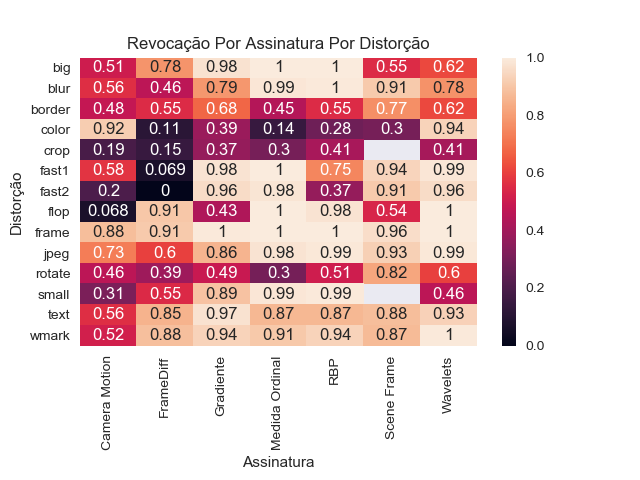
\includegraphics[width=\textwidth]{dados/figuras/experimentos/heatmap_final_recall.png}	
      \fonte{Autoria própria.}
\end{figure}

As assinaturas temporais (Camera Motion e FrameDiff) obtiveram os piores resultados na análise da robustez em geral, sendo que elas são especialmente afetadas pelas distorções temporais de aceleração fast1 e fast2. É possível notar também que a medida com que os vídeos foram mais acelerados, as assinaturas temporais tiveram resultados piores. A assinatura temporal FrameDiff obteve aproximadamente 6\% no teste com a distorção fast1 e e 0\% com a distorção fast2, mostrando que esse tipo de assinatura é extremamente sensível à perda de informação causada pela diminuição do número de quadros de um vídeo. A Camera Motion foi mais sensível a distorção flop, que inverte o vídeo horizontalmente. Isso faz sentido pois esta distorção inverte a translação e rotação da câmera. A última distorção temporal, frame, foi a que causou menos problemas para as assinaturas em geral (3 delas conseguiram classificar corretamente em 100\% dos casos e todas as outras têm revocação maior que 80\%), pois a quantidade de quadros retirados de um vídeo é pequena se comparado às outras distorções temporais, além disso este tipo de distorção é pouco perceptível por humanos.

Outras distorções que tiveram pouco efeito sobre a classificação são as que adicionam textos de forma uniforme nos vídeos: text e wmark. O único caso em que estas distorções afetaram significativamente a classificação é com a utilização da assinatura Camera Motion. Como ela se baseia no rastreamento do movimento de regiões do vídeo entre os quadros, o posicionamento estático do texto realizado pela distorção o impede de acompanhar os movimentos precisamente.

Entre as distorções fotométricas, a color foi a mais efetiva em enganar a detecção de cópias, apenas as assinaturas Camera Motion e Wavelets conseguiram resultados bom com revocação acima dos 90\%, enquanto todas as outras assinaturas obteram valores de revocação abaixo de 40\%. Os resultados favoráveis a essas duas assinaturas se devem ao fato destas não utilizarem valores de luminância para descrever um vídeo, enquanto os outros o fazem. Já a distorção blur afetou negativamente todos as assinaturas que usam bordas ou pequenas regiões de interesse para descrever um vídeo, pois enfraquece os detalhes de um quadro. A distorção jpeg teve resultados semelhantes por também causar uma perda de informação dentro de cada quadro do vídeo. 

% Por fim, as assinaturas geométricas...
% No geral, a assinatura... para fotométricas, para temporais e geométricas

A revocação sozinha não pode ser utilizada para a avaliação de uma assinatura, pois bastaria marcar todos os pares de vídeos como sendo cópias para atingir um valor de 100\% de revocação. Vê-se necessária uma análise complementar à da robustez, sobre a capacidade discriminante de uma assinatura: a unicidade. A seção a seguir discute sua definição, apresenta uma forma de medi-la e avalia cada assinatura quanto a essa métrica.

% Verificar se consegue encontrar a cópia
\section{Unicidade}

Segundo \citeonline{hua2004robust}, unicidade é a capacidade discriminativa de uma assinatura de vídeo, o que significa que vídeos com conteúdos diferentes devem ter assinaturas diferentes. Esta característica é essencial para a utilidade de uma assinatura, pois uma técnica que gera muitos casos de falsos positivos perde sua utilidade como ferramenta de automação de detecção de cópias. Para avaliar esta característica, é utilizada a medida de precisão, que mede a quantidade de casos que são relevantes (verdadeiros positivos), dentro de todos os pares de vídeos que são classificados como cópias (verdadeiros positivos e falsos positivos)\cite{Ting2010}.

\begin{figure}[h]
	\centering
	\caption{Mapa de calor de precisão de cada tipo de assinatura com cada tipo de distorção.}
	\label{fig:heatmap-precisao}
	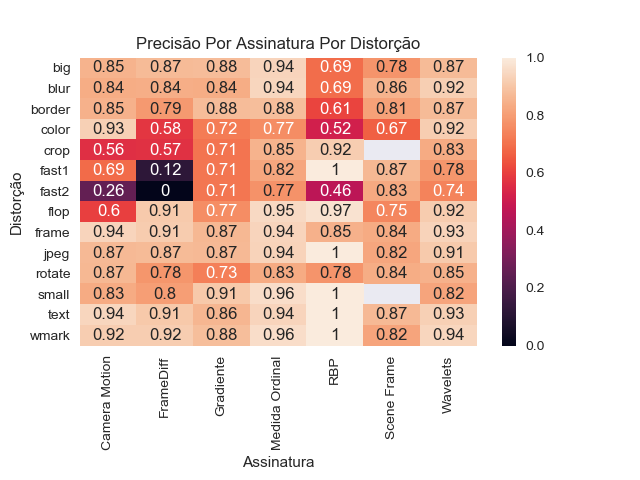
\includegraphics[width=\textwidth]{dados/figuras/experimentos/heatmap_final_precisao.png}
    \fonte{Autoria própria.}
\end{figure}

A Figura~\ref{fig:heatmap-precisao} apresenta os valores de precisão resultados dos testes com todas as assinaturas. Em termos gerais, a assinatura Medida Ordinal tem os melhores resultados neste teste, não apresentando nenhum valor de precisão abaixo de 75\% e tendo valores acima de 90\% para 8 das 14 distorções. Assim como no análise da robustez, as assinaturas temporais obtiveram os piores resultados e o fizeram exatamente nos mesmos casos: fast1, fast2 e flop. 

Para entender o motivo destes resultados para as assinaturas temporais e verificar se estes não se devem a uma escolha ruim de limiares, foram plotados histogramas dos resultados das comparações de cada tipo de assinatura. A Figura~\ref{fig:histograma-camera-motion} apresenta quatro histogramas de valores resultantes da comparação entre pares de vídeos de teste e vídeos originais para a assinatura Camera Motion. Os casos que são cópias estão marcados de verde, enquanto que os não-cópias estão marcados de azul. Quanto mais afastados os dois grupos, maior o poder de discriminação da assinatura para aquela distorção. Nota-se que para a distorção color, a assinatura é capaz de separar os grupos de cópia e não cópia, enquanto que para as outras distorções a assinatura sobrepõe os dois grupos de forma que não é possível separá-los apenas utilizando um limiar de corte. O mesmo ocorre com a assinatura FrameDiff, que não é capaz de classificar assinaturas que sofreram as distorções fast1 e fast2, mas consegue classificar quase perfeitamente casos com as distorções flop e frame(Figura~\ref{fig:histograma-framediff}).

\begin{figure}[h]
	\centering
	\caption{Histogramas de resultados de comparações para a assinatura Camera Motion.}
	\label{fig:histograma-camera-motion}
	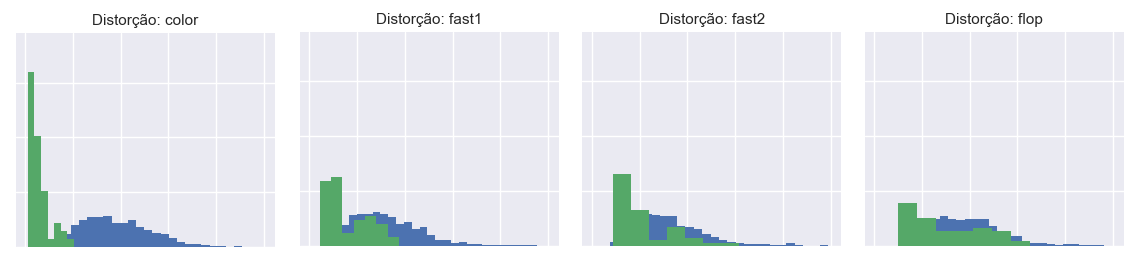
\includegraphics[width=\textwidth]{dados/figuras/experimentos/histograma_distorcao_Camera_Motion_cortado.png}
\end{figure}

\begin{figure}[h]
	\centering
	\caption{Histogramas de resultados de comparações para a assinatura FrameDiff.}
	\label{fig:histograma-framediff}
	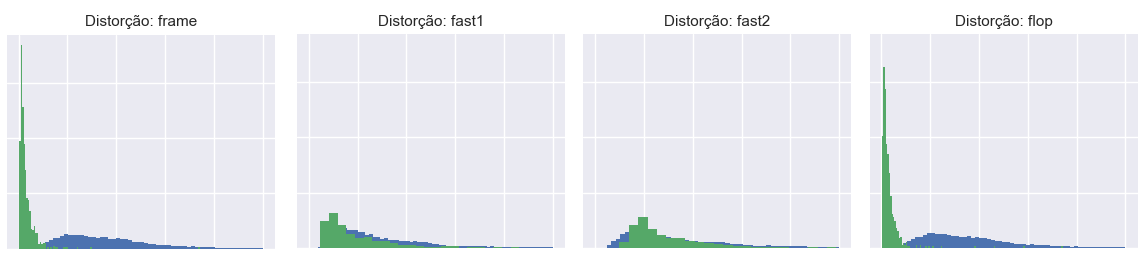
\includegraphics[width=\textwidth]{dados/figuras/experimentos/histograma_distorcao_FrameDiff_cortado.png}
        \fonte{Autoria própria.}
\end{figure}

\section{Peso da escolha do limiar sobre a detecção de cópias}

Para chegar a uma conclusão sobre o tipo de assinatura mais adequado para a detecção de cópias em relação a sua robustez e unicidade, é preciso analisar ambos a precisão e a revocação de forma conjunta. Através da Figura~\ref{fig:heatmap-lado-a-lado} , que compara as duas medidas, nota-se uma relação entre estas: os pontos escuros (piores resultados) estão localizados nas mesmas regiões, mas no geral, todas as assinaturas tiveram resultados de precisão melhores que os de revocação. Além disso, ao observar a figura, nota-se também que a relação entre revocação e precisão não é linear. A Figura~\ref{fig:todos-limiares} mostra a variação das medidas de precisão e revocação a medida que o limiar de corte cresce. Há claramente uma diminuição da capacidade discriminativa de cada assinatura a medida com que o limiar de corte se afasta do zero, e evidencia que cada assinatura apresenta uma proporção diferente para essa diminuição. As assinaturas Medida Ordinal, Wavelets, Scene Frame e RBP são as que mantém a precisão em níveis mais altos. 

\begin{figure}[h]
	\centering
	\caption{Mapas de calor de revocação e precisão para cada assinatura.}
	\label{fig:heatmap-lado-a-lado}
	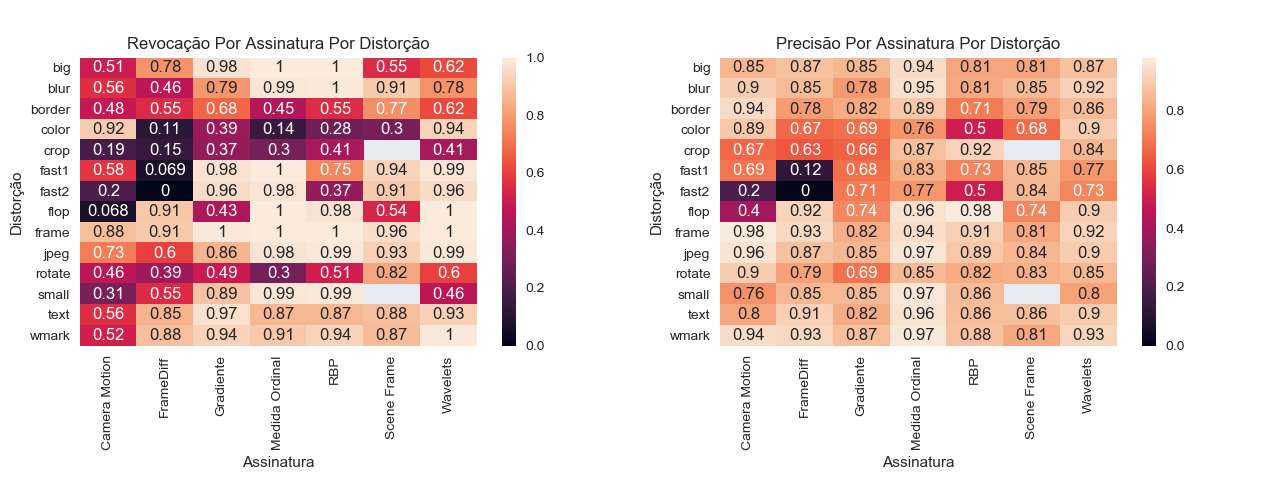
\includegraphics[width=\textwidth]{dados/figuras/experimentos/heatmap_lado.png}
        \fonte{Autoria própria.}
\end{figure}

\begin{figure}[h]
	\centering
	\caption{Simulação de classificação para cada um dos tipos de assinatura. A medida que o limiar se afasta do zero, o valor de precisão diminui e o de revocação aumenta. Cada tipo de assinatura tem uma proporção diferente para essa variação.}
	\label{fig:todos-limiares}
	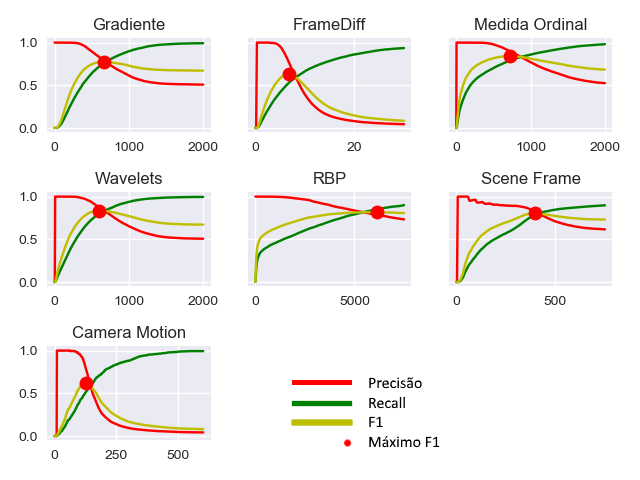
\includegraphics[width=\textwidth]{dados/figuras/experimentos/todos_final.png}
    \fonte{Autoria própria.}
\end{figure}
 
A seguir, será discutido se a aplicação de dois tipos de assinatura de forma conjunta é mais eficiência na detecção de cópias que a aplicação de apenas uma de forma isolada. Será definido o método de combinação destas assinaturas, além da escolha de um limiar de classificação para cada uma destas combinações.

\section{Combinação de Assinaturas}

Assim como as distorções, as assinaturas podem ser classificadas quanto às características de um vídeo que elas utilizam em sua formação. Das assinaturas usadas neste trabalho, duas são temporais (Camera Motion e FrameDiff), enquanto todas as outras são espaciais. Nesta etapa dos experimentos, estes dois tipos de assinatura foram combinados a fim de definir se as métricas de robustez e unicidade são melhoradas em relação às assinaturas utilizadas separadamente. Embora várias combinações de assinaturas sejam possível, para este trabalho, assinatura Camera Motion foi combinada com as todas as outras. 

O primeiro passo é a definição do método de combinação destas assinaturas. Ao invés de combinar os vetores de assinaturas em si, são combinados os valores de distância retornados ao passar um par de vetores pelo DTW, a fim de criar um valor de distância que é a soma ponderada dos valores originais, como mostra a fórmula a seguir.

$$
Dist_{final} = Dist_{ass1} * \alpha + Dist_{ass2} * (1-\alpha)
$$

Como cada tipo de assinatura gera valores muito diferentes ao ser usado como entrada para o DTW (veja Tabela~\ref{tab:limiares} para exemplos), esses valores passam por uma etapa de normalização antes de serem combinados. Além disso, é preciso escolher o fator $\alpha$ de combinação, além de definir um novo limiar de classificação para a "nova assinatura" criada. Assim como para a análise dos algoritmos separados no início deste capítulo, foi realizada uma simulação de classificação com um intervalo de valores de limiares, a fim de definir um limiar para a classificação maximizando a medida fmeasure. Essa simulação foi repetida para os valores de $\alpha = \{0.1, 0.25, 0.5, 0.75, 0.9\}$, como ilustra a Figura~\ref{fig:alpha-limiar}. Os resultados da etapa de parametrização estão dispostos na Tabela~\ref{tab:juncao-limiares-alpha}.

\begin{figure}[h]
	\centering
	\caption{Simulação de classificação todas as combinações de assinatura, alternando o valor de alpha entre 0.1 e 0.9.}
	\label{fig:alpha-limiar}
	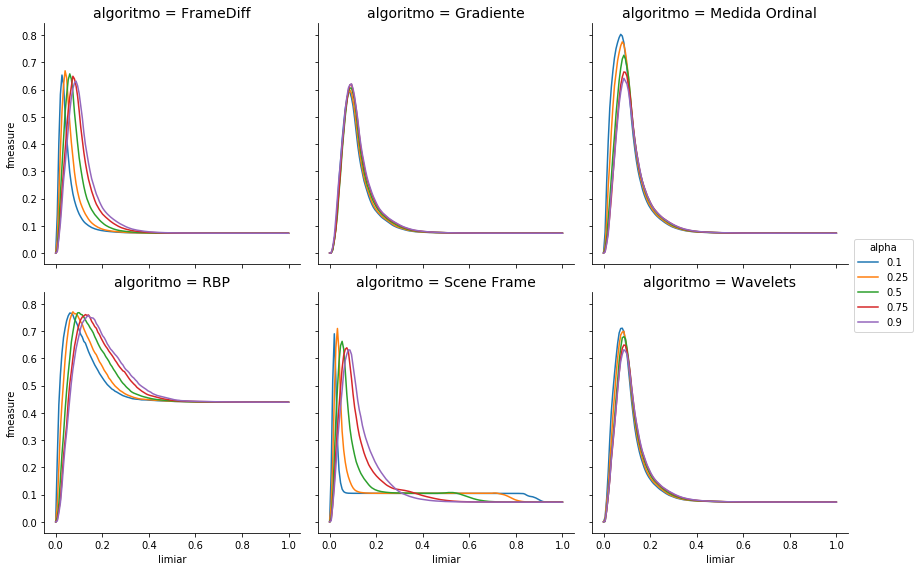
\includegraphics[width=\textwidth]{dados/figuras/experimentos/alpha_juncao.png}
    \fonte{Autoria própria.}
\end{figure}

\begin{table}[h]
\centering
\caption{Tabela com os valores de alpha e limiar que maximizam a fmeasure na etapa de parametrização.}
\label{tab:juncao-limiares-alpha}
\begin{tabular}{|l|l|r|r|r|}
\hline
\textbf{Assinatura 1} & \textbf{Assinatura 2} & \textbf{Alpha} & \textbf{Limiar} & \textbf{Fmeasure} \\\hline
\multirow{6}{*}{Camera Motion} & FrameDiff & 0.25 & 0.040268 & 0.668909 \\\cline{2-5}
& Gradiente & 0.90 & 0.093960 & 0.620811 \\\cline{2-5}
& Medida Ordinal & 0.10 & 0.073826 & 0.802687 \\\cline{2-5}
& RBP & 0.25 & 0.073826 & 0.771050 \\\cline{2-5}
& Scene Frame & 0.25 & 0.033557 & 0.709924 \\\cline{2-5}
& Wavelets & 0.10 & 0.080537 & 0.710831 \\\hline
	\end{tabular}
    \fonte{Autoria própria.}
\end{table}

Após a etapa de parametrização, foram rodados os testes utilizando os valores de $\alpha$ e de limiar definidos anteriormente. Para comparar os resultados com aqueles dos algoritmos separados, os valores da medida fmeasure para cada teste de classificação estão dispostos na Figura~\ref{fig:compacao-metodos}. No geral, a combinação de duas assinaturas não teve efeitos positivos na classificação. Com ela, todas as combinações passaram a ser sensíveis a distorções temporais e poucos casos apresentaram melhoras. Nos casos em que a mudança foi positiva, o ganho foi de menos de 5\%. 

\begin{figure}
	\caption{Histograma com valores de fmeasure para cada tipo de assinatura. A esquerda, resultados da combinação da assinatura Camera Motion com as demais, a direita, assinaturas aplicadas isoladamente.}
	\label{fig:compacao-metodos}
	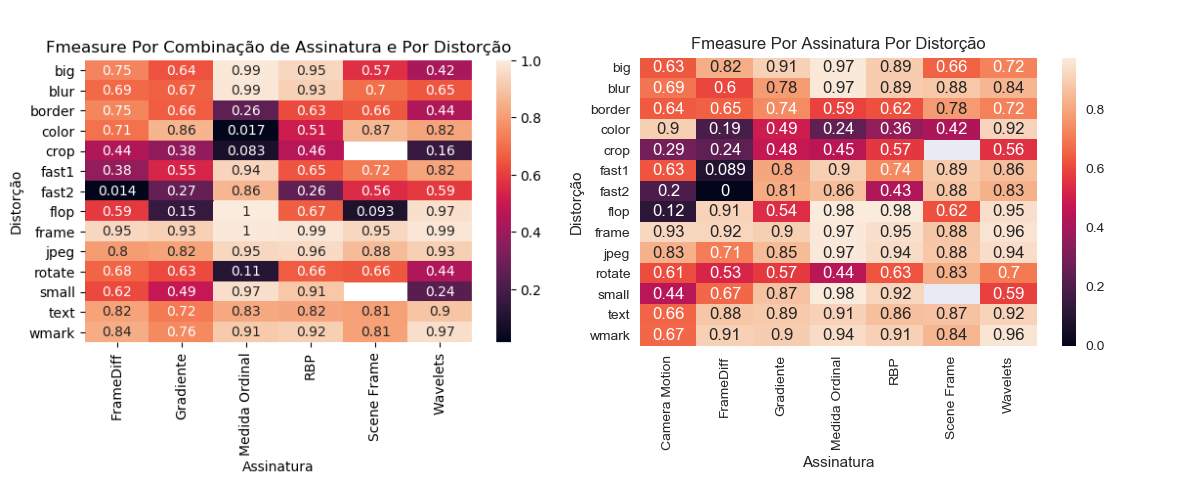
\includegraphics[width=\textwidth]{dados/figuras/experimentos/heatmap_final_comparacao.png}
    \fonte{Autoria própria.}
\end{figure}

% Por fim, para avaliar as assinaturas de modo geral, é preciso levar em consideração sua robustez e unicidade simultaneamente. 

% \begin{figure}[h]
% 	\centering
% 	\caption{Mapa de calor de \textit{fmeasure} de cada tipo de assinatura com cada tipo de distorção}
% 	\label{fig:heatmap-final_f1}
% 	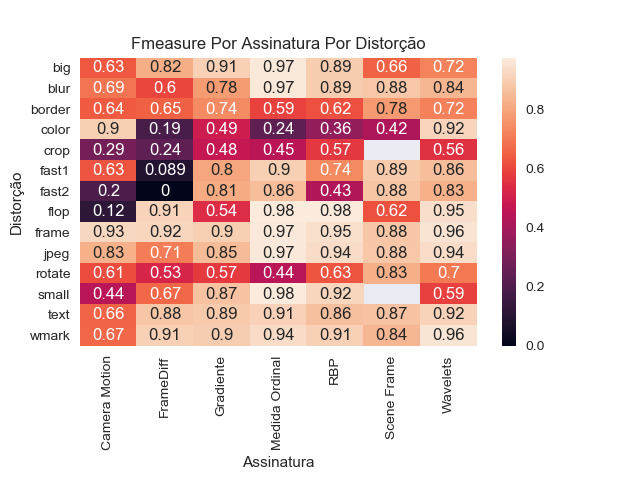
\includegraphics[width=\textwidth]{dados/figuras/experimentos/heatmap_final_f1.png}
% \end{figure}


% Verificar se identifica que é cópia de apenas 1 vídeo

% Separar por distorções e discutir o resultado de cada algoritmo
% Mostrar que 

% ------------------------- Treinamento
% \begin{figure}[h]
% 	\centering
% 	\label{fig:limiares-framediff}
% 	\caption{Teste de limiares para a assinatura framediff}
% 	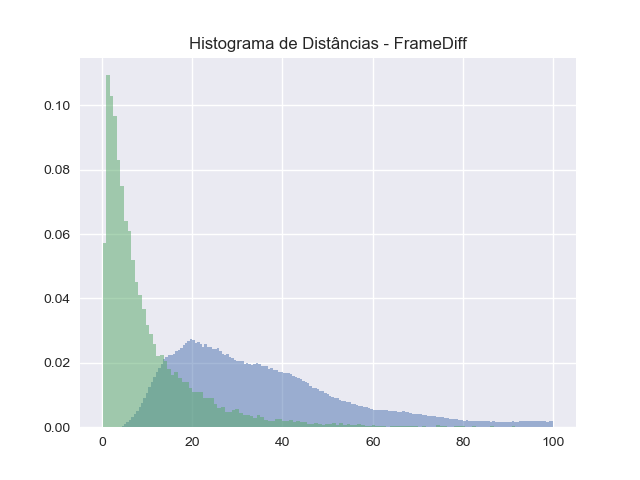
\includegraphics[width=0.8\textwidth]{dados/figuras/experimentos/histograma_FrameDiff.png}
% \end{figure}
% \begin{figure}[h]
% 	\centering
% 	\label{fig:limiares-medidaordinal}
% 	\caption{Teste de limiares para a assinatura medida ordinal}
% 	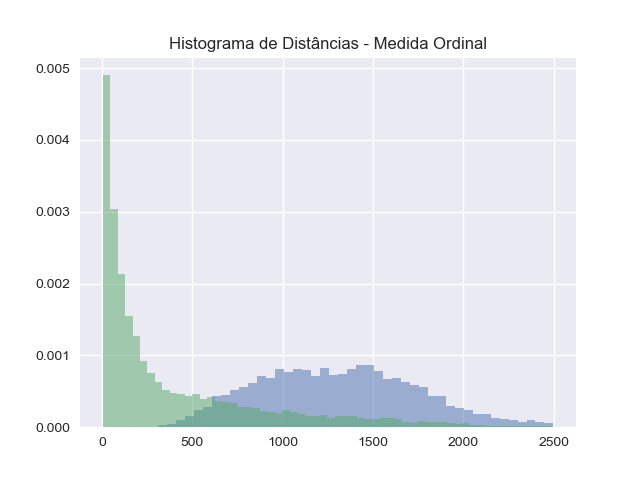
\includegraphics[width=0.8\textwidth]{dados/figuras/experimentos/histograma_Medida_Ordinal.png}
% \end{figure}
% \begin{figure}[h]
% 	\centering
% 	\label{fig:limiares-sceneframe}
% 	\caption{Teste de limiares para a assinatura sceneframe}
% 	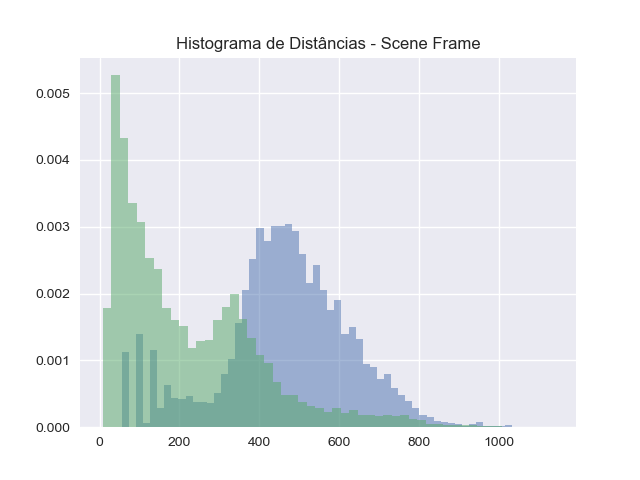
\includegraphics[width=0.8\textwidth]{dados/figuras/experimentos/histograma_Scene_Frame.png}
% \end{figure}
% \begin{figure}[h]
% 	\centering
% 	\label{fig:limiares-gradiente}
% 	\caption{Teste de limiares para a assinatura gradiente}
% 	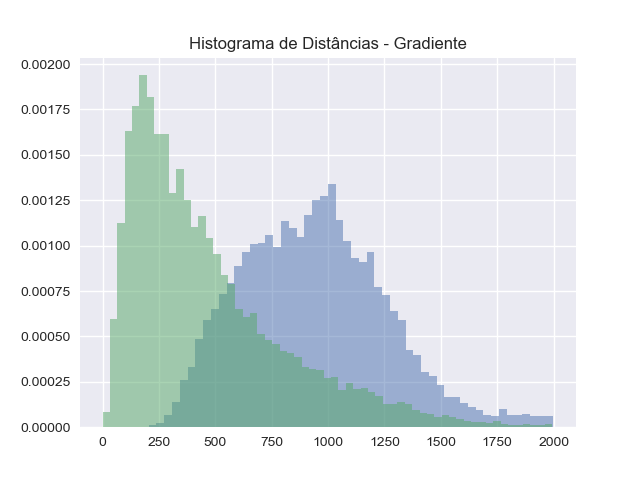
\includegraphics[width=0.8\textwidth]{dados/figuras/experimentos/histograma_Gradiente.png}
% \end{figure}
% \begin{figure}[h]
% 	\centering
% 	\label{fig:limiares-rbp}
% 	\caption{Teste de limiares para a assinatura rbp}
% 	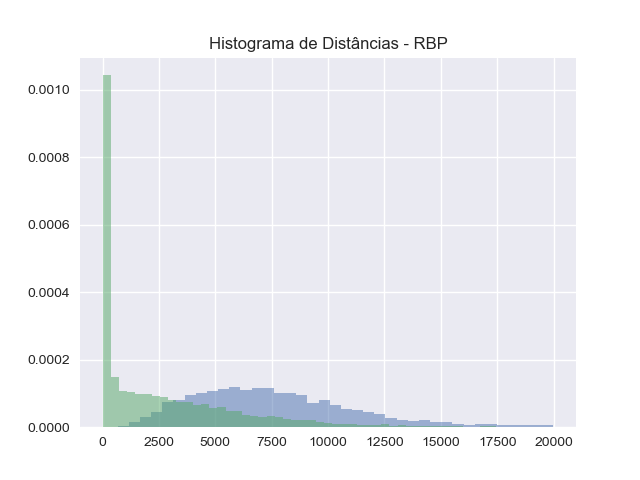
\includegraphics[width=0.8\textwidth]{dados/figuras/experimentos/histograma_RBP.png}
% \end{figure}
% \begin{figure}[h]
% 	\centering
% 	\label{fig:limiares-wavelets}
% 	\caption{Teste de limiares para a assinatura wavelets}
% 	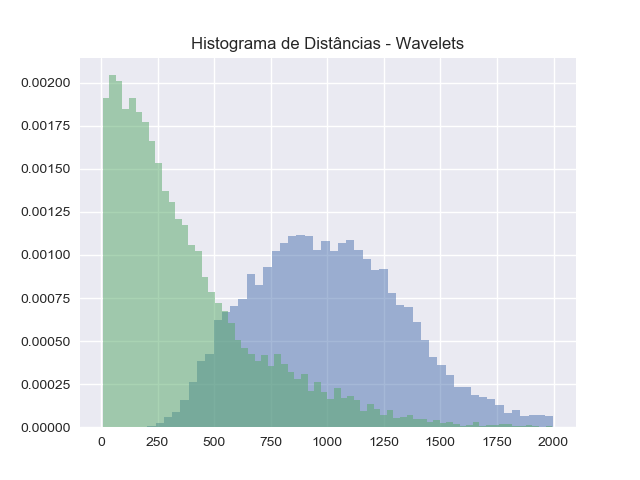
\includegraphics[width=0.8\textwidth]{dados/figuras/experimentos/histograma_Wavelets.png}
% \end{figure}

% \begin{figure}[h]
% 	\centering
% 	\label{fig:limiares-camera-motion}
% 	\caption{Teste de limiares para a assinatura camera motion}
% 	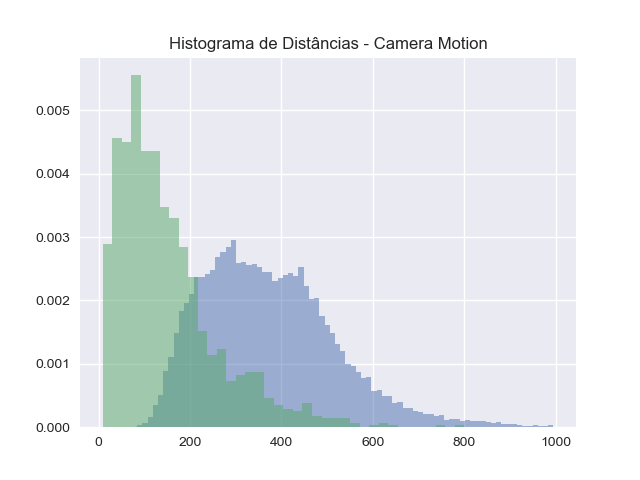
\includegraphics[width=0.8\textwidth]{dados/figuras/experimentos/histograma_Camera_Motion.png}
% \end{figure}

% \begin{figure}[h]
% 	\centering
% 	\label{fig:limiares}
% 	\caption{Limiares}
% 	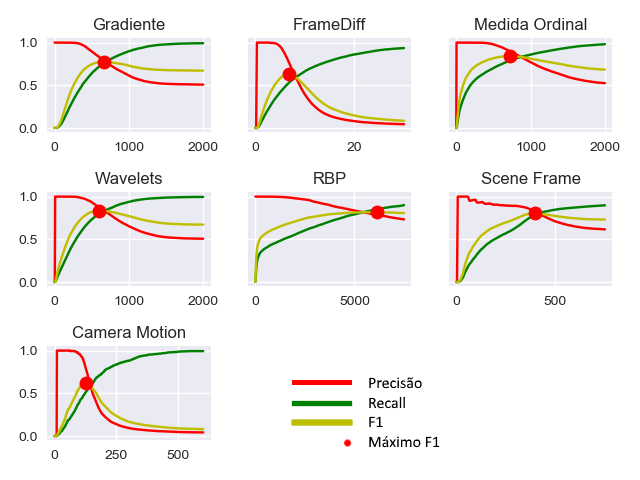
\includegraphics[width=\textwidth]{dados/figuras/experimentos/todos_final.png}
% \end{figure}

% \begin{figure}[h]
% 	\centering
% 	\label{fig:final_heatmap}
% 	\caption{Final}
% 	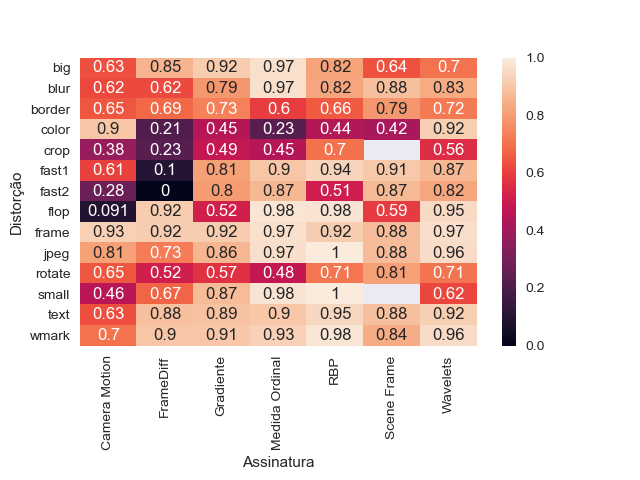
\includegraphics[width=\textwidth]{dados/figuras/experimentos/heatmap_final.png}
% \end{figure}


% \begin{figure}[h]
% 	\centering
% 	\label{fig:limiares-framediff}
% 	\caption{Teste de limiares para a assinatura framediff}
% 	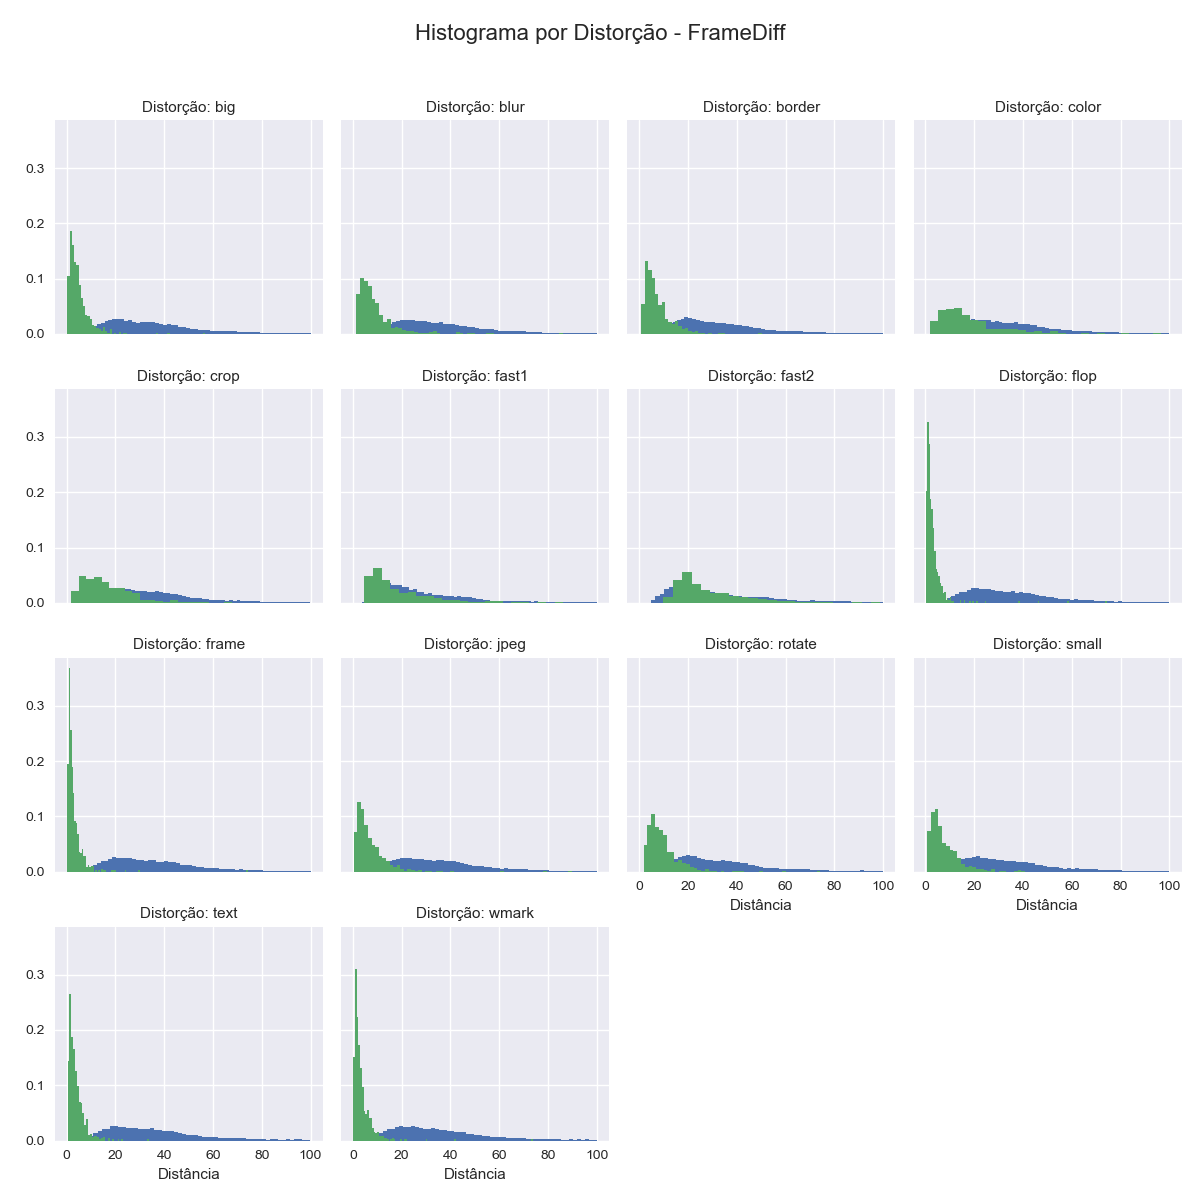
\includegraphics[width=\textwidth]{dados/figuras/experimentos/histograma_distorcao_FrameDiff.png}
% \end{figure}
% \begin{figure}[h]
% 	\centering
% 	\label{fig:limiares-medidaordinal}
% 	\caption{Teste de limiares para a assinatura medida ordinal}
% 	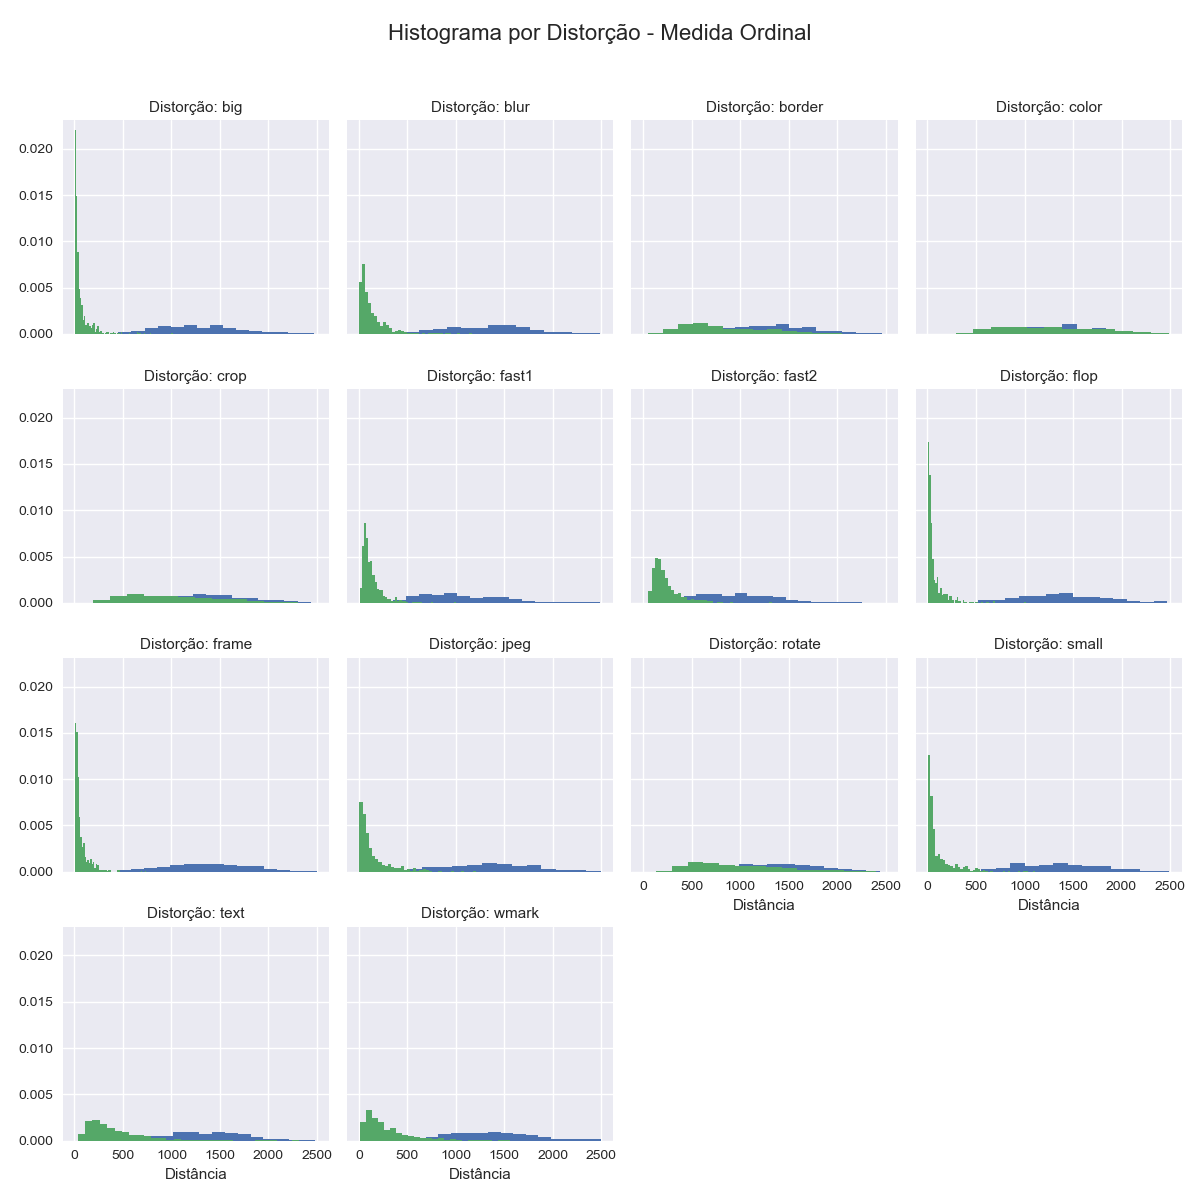
\includegraphics[width=\textwidth]{dados/figuras/experimentos/histograma_distorcao_Medida_Ordinal.png}
% \end{figure}
% \begin{figure}[h]
% 	\centering
% 	\label{fig:limiares-sceneframe}
% 	\caption{Teste de limiares para a assinatura sceneframe}
% 	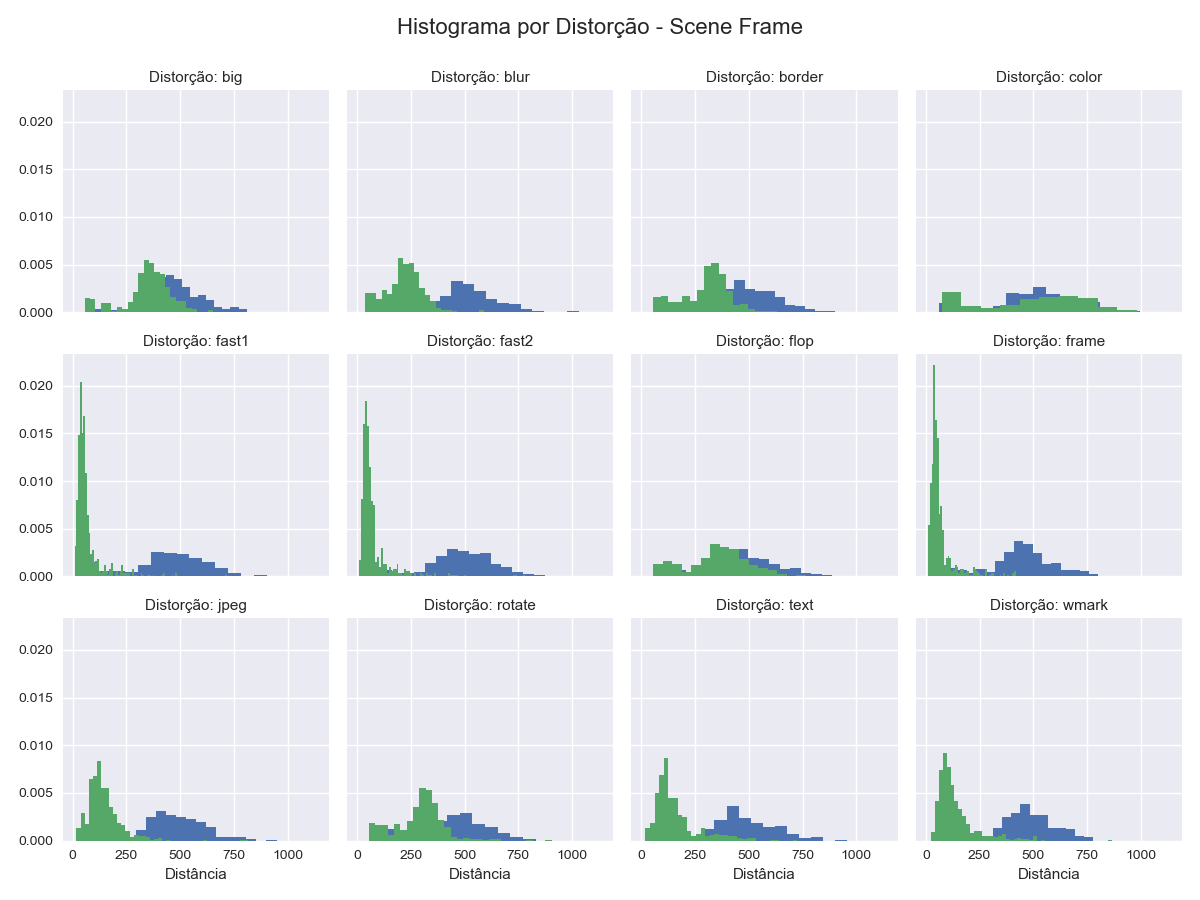
\includegraphics[width=\textwidth]{dados/figuras/experimentos/histograma_distorcao_Scene_Frame.png}
% \end{figure}
% \begin{figure}[h]
% 	\centering
% 	\label{fig:limiares-gradiente}
% 	\caption{Teste de limiares para a assinatura gradiente}
% 	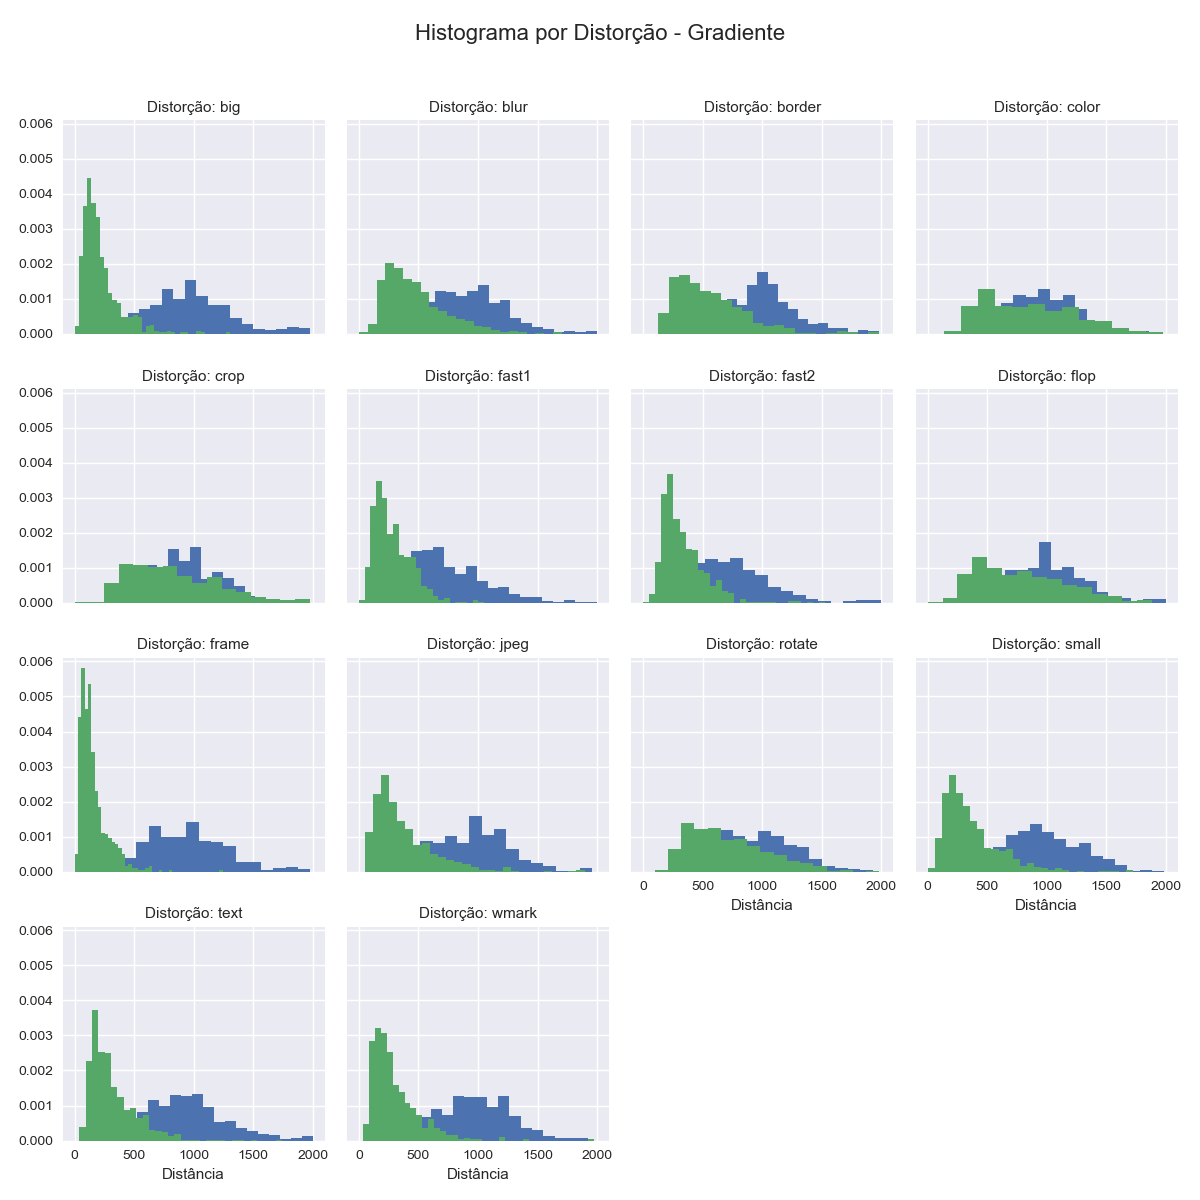
\includegraphics[width=\textwidth]{dados/figuras/experimentos/histograma_distorcao_Gradiente.png}
% \end{figure}
% \begin{figure}[h]
% 	\centering
% 	\label{fig:limiares-rbp}
% 	\caption{Teste de limiares para a assinatura rbp}
% 	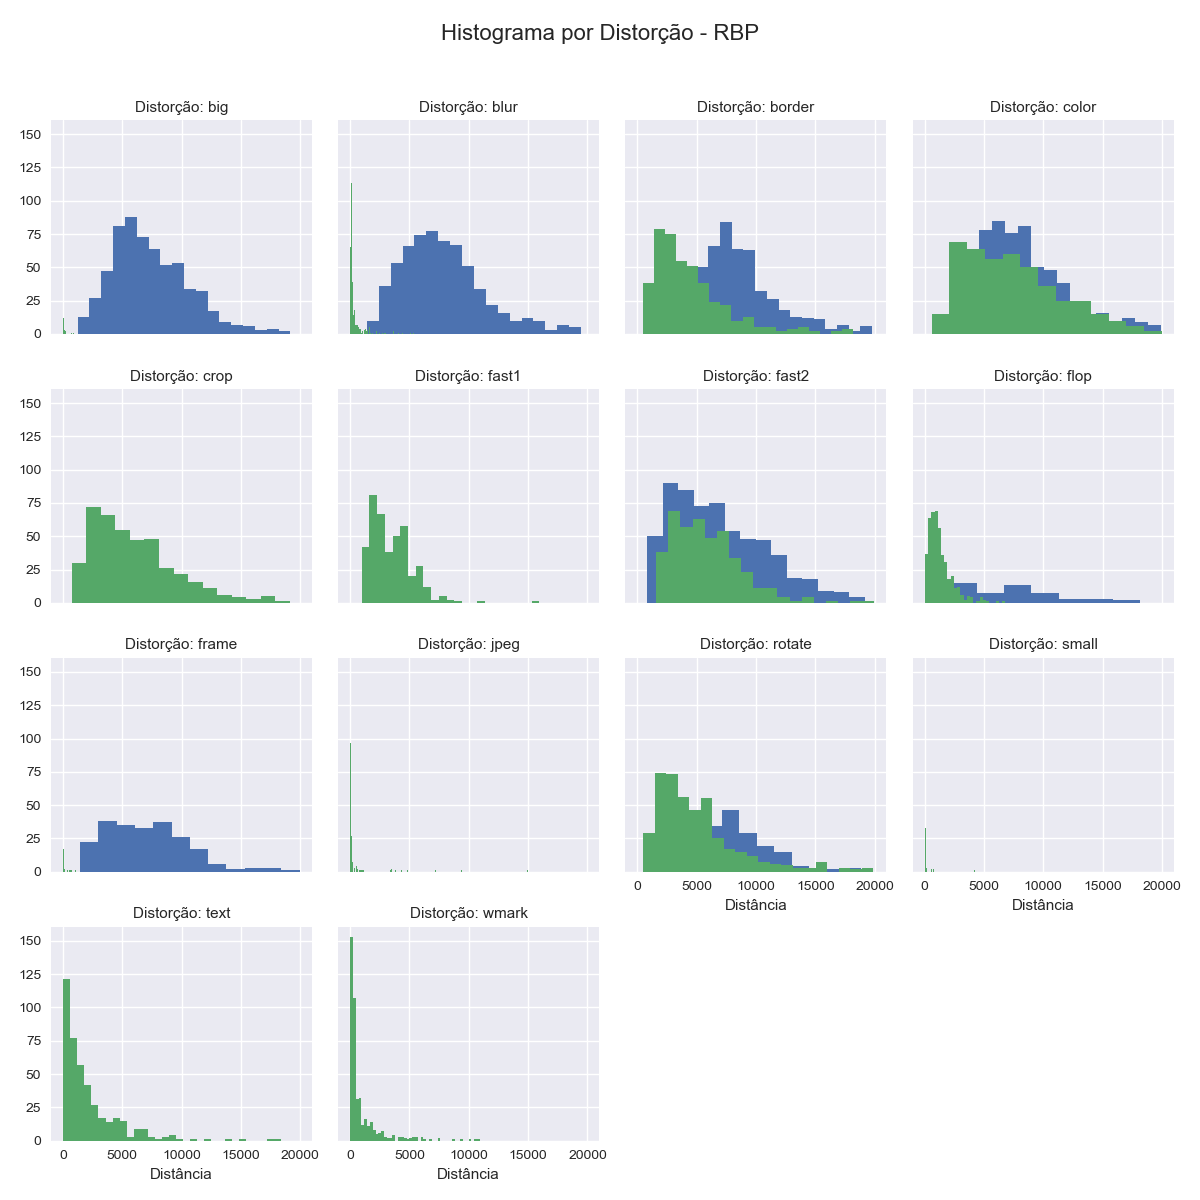
\includegraphics[width=\textwidth]{dados/figuras/experimentos/histograma_distorcao_RBP.png}
% \end{figure}
% \begin{figure}[h]
% 	\centering
% 	\label{fig:limiares-wavelets}
% 	\caption{Teste de limiares para a assinatura wavelets}
% 	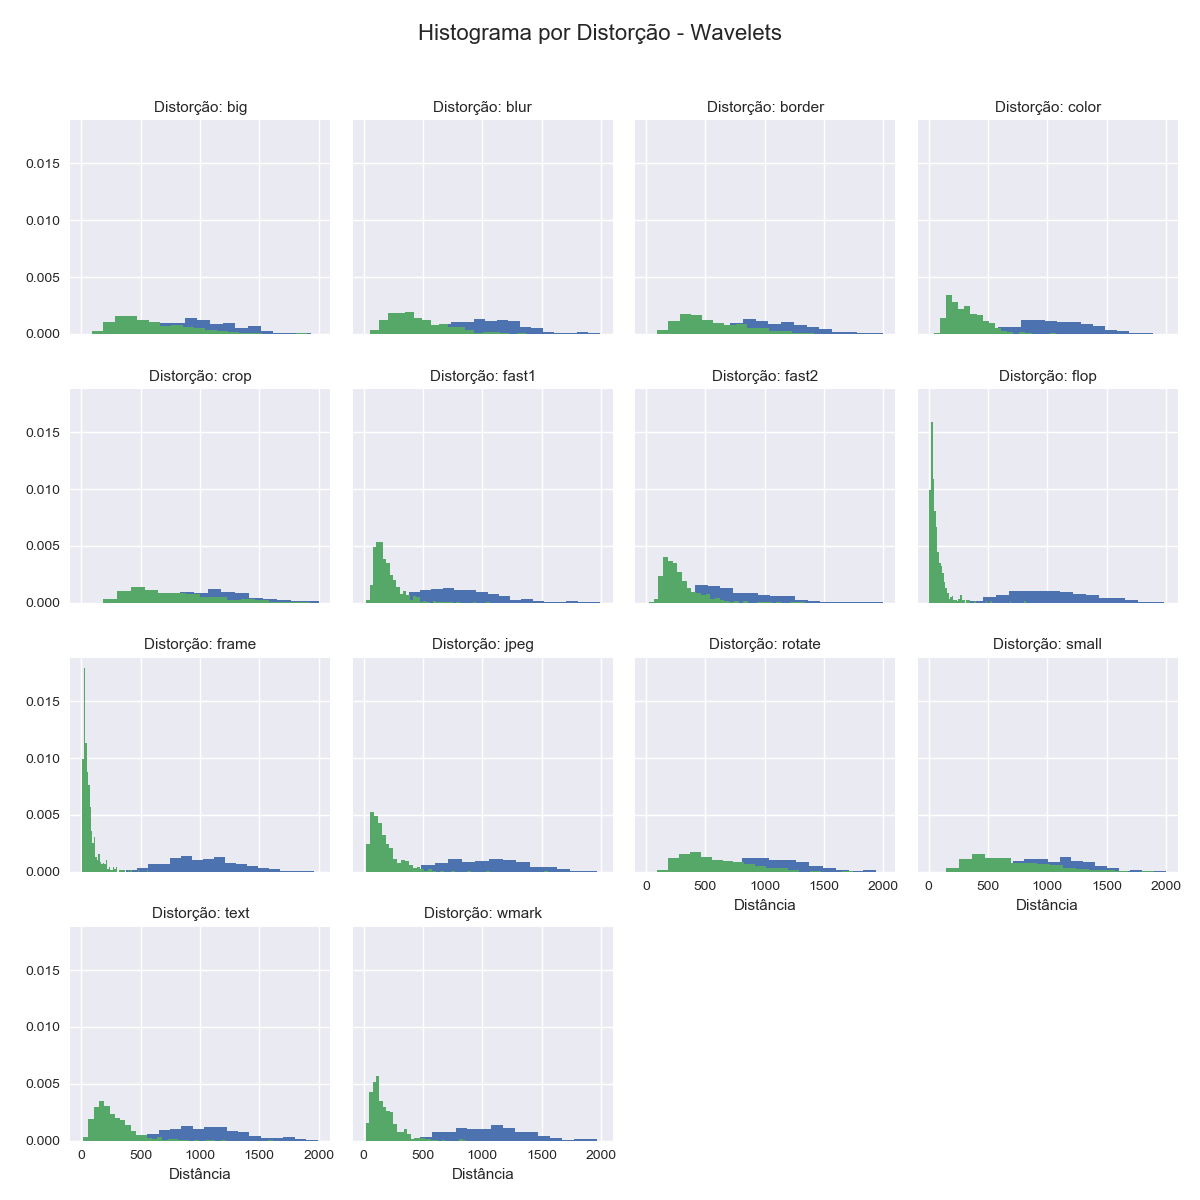
\includegraphics[width=\textwidth]{dados/figuras/experimentos/histograma_distorcao_Wavelets.png}
% \end{figure}

% \begin{figure}[h]
% 	\centering
% 	\label{fig:limiares-camera-motion}
% 	\caption{Teste de limiares para a assinatura camera motion}
% 	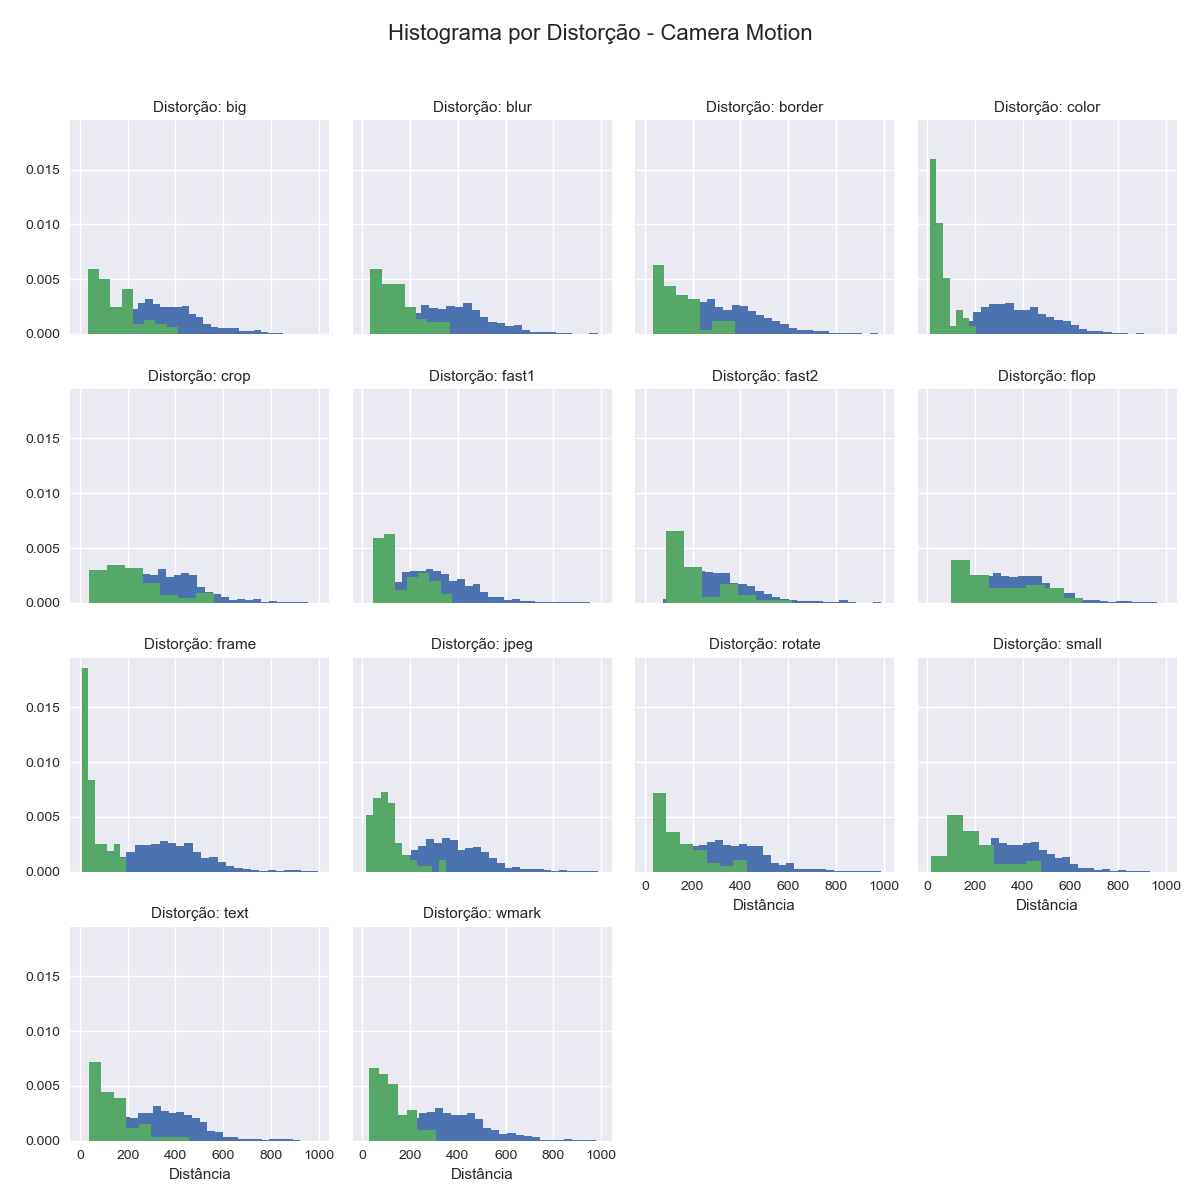
\includegraphics[width=\textwidth]{dados/figuras/experimentos/histograma_distorcao_Camera_Motion.png}
% \end{figure}
